%**************************************************************************
%                                        PLANTILLA PARA REPORTE DE SECO
%**************************************************************************
\documentclass[final]{beamer}

% ====================
% Paquetes
% ====================

\usepackage[T1]{fontenc}
\usepackage{lmodern}
\usepackage[size=custom,width=120,height=86,scale=1.0]{beamerposter}
\usetheme{gemini}
\usecolortheme{uci}  % or uci_dark
\usepackage{graphicx}
\usepackage{booktabs}
\usepackage{tikz}
\usepackage{pgfplots}
\pgfplotsset{compat=1.14}
\usepackage{anyfontsize}

% ====================
% Lengths
% ====================

% If you have N columns, choose \sepwidth and \colwidth such that
% (N+1)*\sepwidth + N*\colwidth = \paperwidth
\newlength{\sepwidth}
\newlength{\colwidth}
\setlength{\sepwidth}{0.025\paperwidth}
\setlength{\colwidth}{0.3\paperwidth}

\newcommand{\separatorcolumn}{\begin{column}{\sepwidth}\end{column}}

% ====================
% Titulo
% ====================

\title{Boletin del Sector Café en Honduas}

\author{Autor \inst{1} \and Autor \inst{2} \and Autor \inst{3}}

\institute[shortinst]{\inst{1} Grupo Financiero Ficohsa \samelineand \inst{2} Riesgos}

% ====================
% Footer (optional)
% ====================

\footercontent{
  \href{https://www.ficohsa.hn/}{https://www.ficohsa.hn/} \hfill
  Gestión Integral de Riesgos \hfill
  \href{Ciencia de datos}{Ciencia de Datos}}
% (can be left out to remove footer)

% ====================
% Body
% ====================

\begin{document}

% Refer to https://github.com/k4rtik/uchicago-poster
% logo: https://www.cam.ac.uk/brand-resources/about-the-logo/logo-downloads
\addtobeamertemplate{headline}{}
{
    \begin{tikzpicture}[remember picture,overlay]
      \node [anchor=north west, inner sep=3cm] at ([xshift=0.0cm,yshift=0.5cm]current page.north west)
      {
\includegraphics[height=3.5cm]{logos/logo.png}};
      % {\includegraphics[height=3.5cm]{logos/university-of-california-irvine-uci-vector-logo-wordmark-white.eps}};
    \end{tikzpicture}
}

\begin{frame}[t]
\begin{columns}[t]
\separatorcolumn

\begin{column}{\colwidth}

%====================================================
%                                                        BLOQUE 1
%====================================================
  \begin{block}{Contexto general}

    El \textbf{sector cafetalero hondureño} continúa siendo uno de los pilares de la economía nacional, representando aproximadamente el 5\% \textbf{del PIB total} y cerca del 20\% \textbf{del PIB agrícola}. Además, genera más de \textbf{120 mil empleos directos} y constituye la \textbf{principal fuente de divisas del sector agroexportador.}\\[0.4cm]

   Sin embargo, el entorno actual presenta \textbf{retos significativos}. Tras alcanzar un récord histórico de \textbf{7.29 millones de sacos exportados en la cosecha de 2016-2017}, el volumen cayo a \textbf{4.68 millones de sacos en la cosecha 2023-2024}, lo que equivale a una \textbf{reducción del 36\%}. Esta contracción responde a una combinación de factores como la \textbf{volatilidad en los precios internacionales, condiciones climáticas adversas} y \textbf{aumentos en los costos de producción y transporte}.  
   
   \begin{center}
    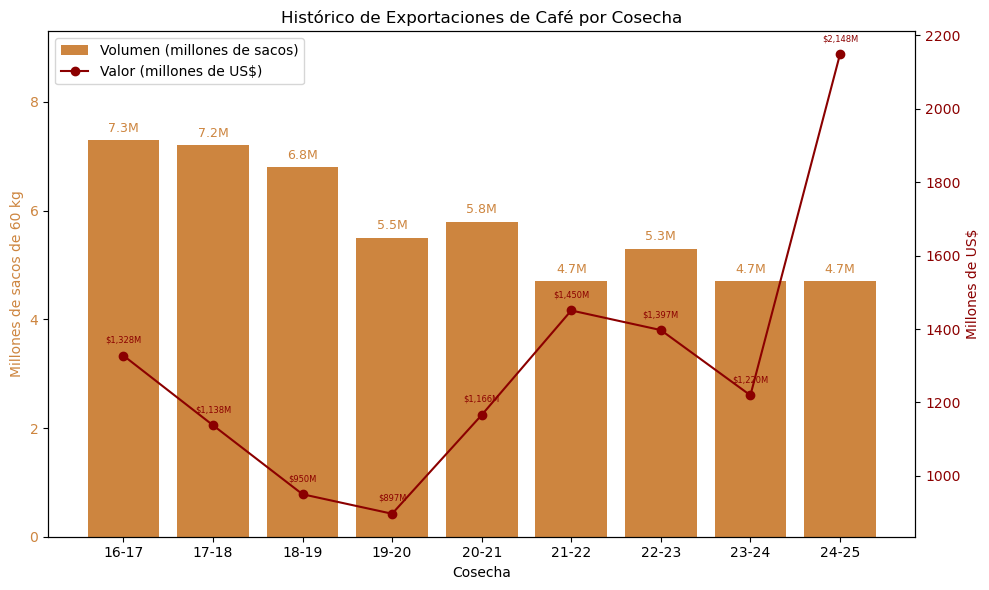
\includegraphics[scale=0.55]{C:/Users/HN32885/Documents/2025/LateX/PPT_Beamer_Sectores/fig1.jpg}
   \end{center}

Al mismo tiempo, las \textbf{expectativas de precios futuros} muestran signos mixtos: mientras los contratos en la bolsa de Nueva York (ICE Coffe C) se mantienen por encima del promedio histórico, los \textbf{margenes de rentabilidad del productor} se han visto presionados por la inflación y la apreciación del dólar.\\[0.4cm]

En este boletín, elaborado por el área de \textbf{Gestión Integral de Riesgos} y \textbf{Ciencia de Datos de Grupo Financiero Ficohsa}, se analiza la \textbf{coyuntura actual del sector café}, sus principales \textbf{riesgos microfinancieros} y la \textbf{calificación del sector según el modelo IRSS (Índice de Riesgos Sectorial Sistématico)}, con el fin de apoyar la \textbf{toma de decisiones estratégicas de crédito y apetito de riesgo} institucional.

  \end{block}
%====================================================
%                                                        BLOQUE 2
%====================================================
  \begin{block}{Desempeño reciente del sector cafetalero}

De acuerdo con datos de ADECAFEH e IHCAFE, durante la cosecha 2023-2024 las exportaciones de café hondureño se estabilizaron en torno a \textbf{4.68 millones de sacos de 60kg}, cifra que confirma la \textbf{moderación en la producción} tras varios años de ajustes estructurales en el sector. Aunque el volumen continúa por debajo del máximo histórico alcanzado en 2016-2017, el \textbf{valor exportado mostró una recuperación parcial} gracias a mejores precios internacionales y a una \textbf{mayor participación de cafés diferenciados (orgánico, RFA, FLO, entre otros).}\\[1cm]

El repunte observado en el valor de exportación responde principalmente a \textbf{factores de mercado externos}, más que aun aumento en la productividad local, lo cual mantiene al sector \textbf{expuesto a la volatilidad de precios} y a las \textbf{condiciones climáticas} que afectan la oferta mundial. \\[1cm]

En este contexto, el \textbf{IRSS}, modelo desarrollado por el área Gestión Integral de Riesgos y Ciencia de Datos permite \textbf{cuantificar el nivel de vulnerabilidad y estabilidad relativa} del sector frente a factores macroeconómicos, financieros y productivos. \\[1cm]

Según la estimación más reciente, el IRSS del sector café se ubica en XXXXXX (nivel bajo), lo que refleja una exposición baja al riesgo sistémico, sustentada en precios favorables pero con alta sensibilidad a choques externos.

   

  \end{block}
%====================================================
%                                                        BLOQUE 3
%====================================================
  \begin{block}{Factores macroeconómicos y exposición crediticia}

{Según el IRSS, el comportamiento de ciertos indicadores o variables condiciona directamente la capacidad de pago del sector cafetalero y el nivel de riesgo que asume el banco al otorgar créditos agrícolas. Estas variables son: }
{\small
\begin{itemize}
\item \textbf{VENTA\_ENERGIA:} ventas de energia de la ENEE.
\item \textbf{SPI3\_ELPA:} índice de precipitaciones acumulado de 3 meses en el Paraíso.
\item \textbf{SPI3\_AGA:} índice de precipitaciones acumulado de 3 meses en Agalta.
\item \textbf{WTI14:} Precio global actual del petróleo.
\item \textbf{IPI\_USA:} índice de producción industrial USA.
\item \textbf{REAL\_EX\_BR:} Tipo de cambio real del real brasileño.
\item \textbf{X\_CAFE\_BR:} Exportaciones de café de Brasil.
\item \textbf{PCA1\_xcafé:} Componente principal o índice sintético de las exportaciones de café.
\end{itemize}
}
{ Estas variables permiten capturar los efectos combinados de la demanda energética, el clima, la producción internacional y las condiciones cambiarias sobre el desempeño del sector cafetalero. En conjunto, explican una proporción significativa de la variabilidad del riesgo crediticio observado en el portafolio agrícola de Ficohsa.}
  \end{block}

\end{column}

\separatorcolumn

\begin{column}{\colwidth}
%====================================================
%                                                        BLOQUE 4
%====================================================
  \begin{block}{Resultados del modelo IRSS y análisis de riesgo}



  \end{block}
%====================================================
%                                                        BLOQUE 4
%====================================================
  \begin{block}{Bloque 5}

    \begin{figure}
      \centering
      \begin{tikzpicture}
        \begin{axis}[
            scale only axis,
            no markers,
            domain=0:2*pi,
            samples=100,
            axis lines=center,
            axis line style={-},
            ticks=none]
          \addplot[red] {sin(deg(x))};
          \addplot[blue] {cos(deg(x))};
        \end{axis}
      \end{tikzpicture}
      \caption{Another figure caption.}
    \end{figure}

  \end{block}
%====================================================
%                                                        BLOQUE 6
%====================================================
  \begin{block}{Bloque 6}



  \end{block}

\end{column}

\separatorcolumn

\begin{column}{\colwidth}
%====================================================
%                                                        BLOQUE 7
%====================================================
  \begin{exampleblock}{Bloque 7}

    $$
    \int_{-\infty}^{\infty} e^{-x^2}\,dx = \sqrt{\pi}
    $$


  \end{exampleblock}
%====================================================
%                                                        BLOQUE 8
%====================================================
  \begin{block}{Bloque 8}


    \begin{table}
      \centering
      \begin{tabular}{l r r c}
        \toprule
        \textbf{First column} & \textbf{Second column} & \textbf{Third column} & \textbf{Fourth} \\
        \midrule
        Foo & 13.37 & 384,394 & $\alpha$ \\
        Bar & 2.17 & 1,392 & $\beta$ \\
        Baz & 3.14 & 83,742 & $\delta$ \\
        Qux & 7.59 & 974 & $\gamma$ \\
        \bottomrule
      \end{tabular}
      \caption{A table caption.}
    \end{table}

  \end{block}
%====================================================
%                                                        BLOQUE 9
%====================================================
  \begin{block}{References}

    \nocite{*}
    \footnotesize{\bibliographystyle{plain}\bibliography{poster}}

  \end{block}

\end{column}

\separatorcolumn
\end{columns}
\end{frame}

\end{document}
